% Ajustes adicionales para el libro impreso 7"x10"
\usepackage{graphicx}
\usepackage{tikz}
\graphicspath{{../../}}

% Portada: la primera página muestra el cover.png a página completa.
% - Dimensiones EXPLÍCITAS (7in x 10in): \includegraphics con width=\paperwidth
%   falla silenciosamente en xelatex y produce página en blanco.
% - Overlay TikZ en lugar de \newgeometry/\restoregeometry: estos fuerzan saltos
%   de página y desplazan la portada/copyright creando páginas en blanco.
\renewcommand{\maketitle}{%
  \thispagestyle{empty}%
  \begin{tikzpicture}[remember picture, overlay]
    \node[inner sep=0, anchor=north west] at (current page.north west)
      {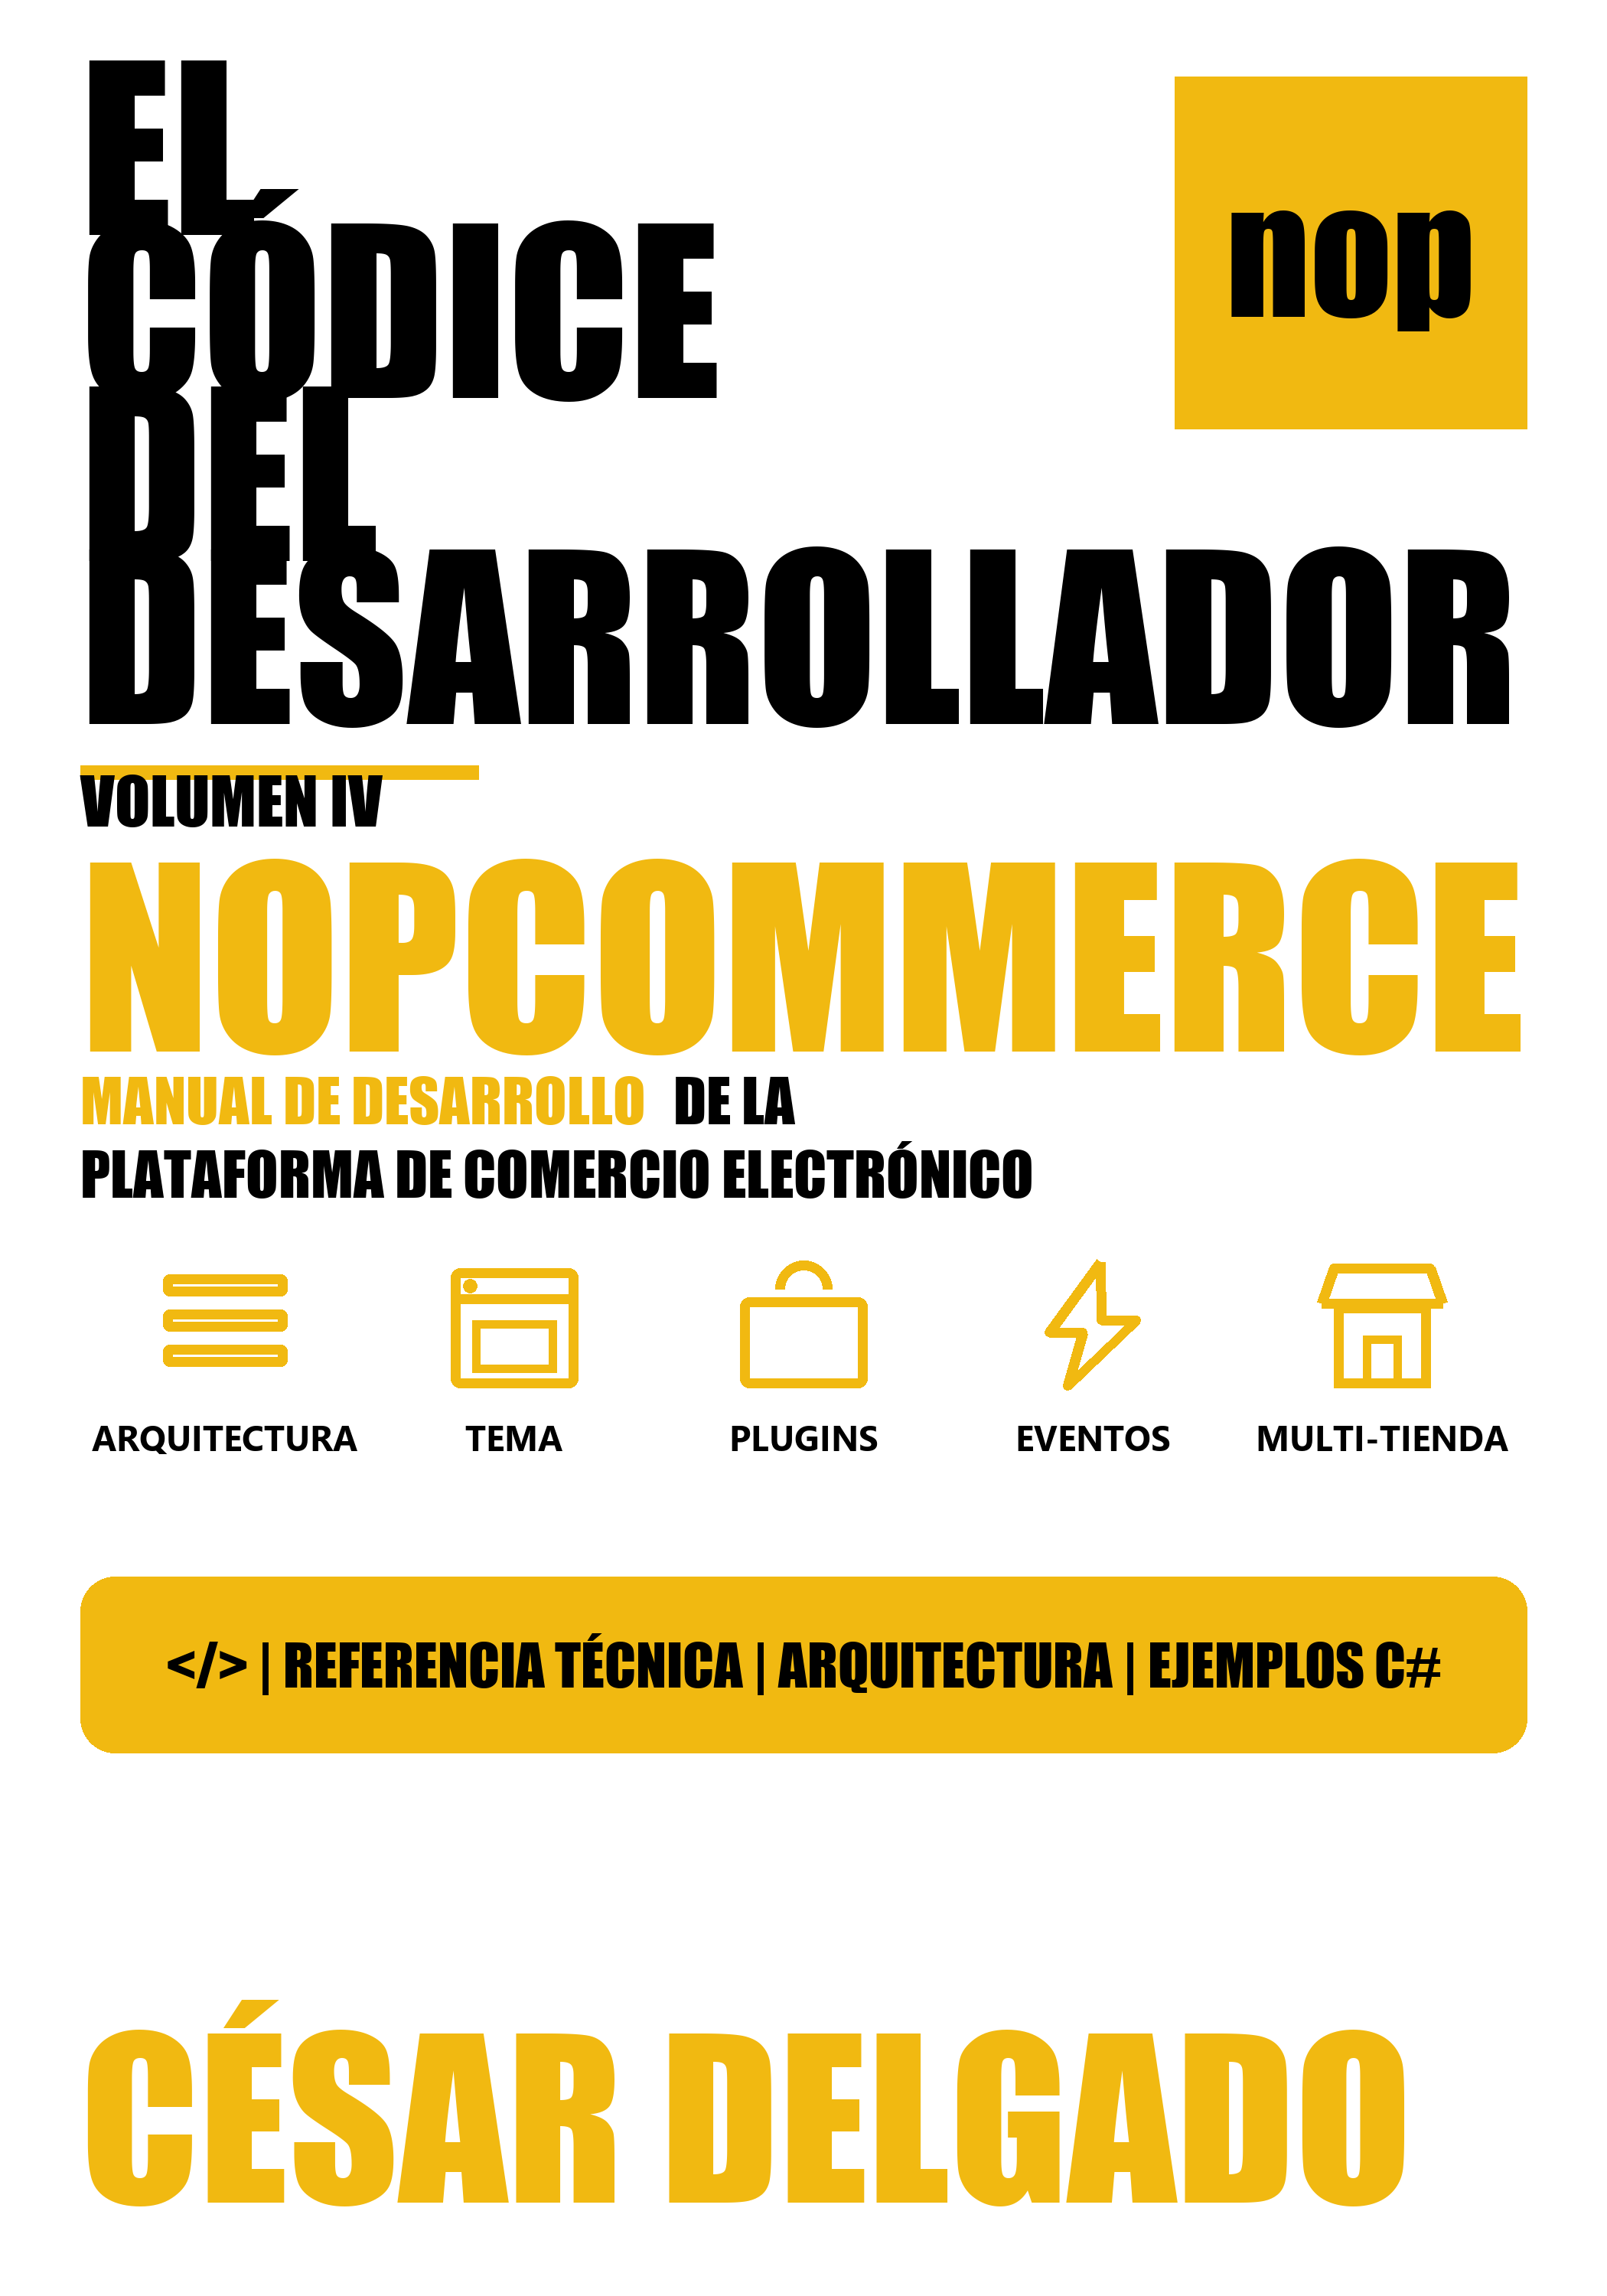
\includegraphics[width=7in,height=10in]{cover.png}};
  \end{tikzpicture}%
  \clearpage
}

\usepackage{fancyhdr}
\pagestyle{fancy}
\fancyhf{}
\fancyhead[LE]{\small\textit{El Códice del Desarrollador}}
\fancyhead[RO]{\small\textit{El Códice del Desarrollador}}
\fancyfoot[C]{\thepage}
\renewcommand{\headrulewidth}{0.4pt}

% Tablas compactas: reducen el tamaño para que quepan en 7"x10"
\AtBeginEnvironment{longtable}{\scriptsize}
\AtBeginEnvironment{tabu}{\scriptsize}
\setlength{\tabcolsep}{3pt}

% Tablas: maquetación unificada con Word y EPUB (MaquetaciónLibroB5.md).
% Cabecera E8E8E8 centrada/negrita y rejilla completa 999999 0,5 pt
% (el filtro filtro_libro.lua construye el longtable con \rowcolor y \hline).
\usepackage{colortbl}
\usepackage{longtable}
\usepackage{array}
\usepackage{calc}
\arrayrulecolor[HTML]{999999}
\setlength{\arrayrulewidth}{0.5pt}

% Permite partir URLs y cadenas largas (texttt) entre líneas
\usepackage{xurl}
\setlength{\emergencystretch}{3em}
\sloppy

% Evita que los bloques de código se corten al cambiar de página
\usepackage{etoolbox}
\BeforeBeginEnvironment{verbatim}{\par\small}
